\documentclass{standalone}
\usepackage{tikz}
\usepackage{basicreq}

\usetikzlibrary{positioning}
\begin{document}

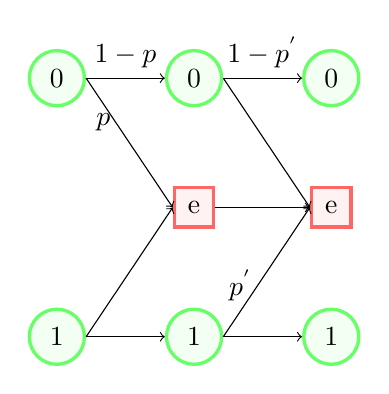
\begin{tikzpicture}[
roundnode/.style={circle, draw=green!60, fill=green!5, very thick, minimum size=7mm},
squarednode/.style={rectangle, draw=red!60, fill=red!5, very thick, minimum size=5mm},
]
%Nodes
\node[roundnode, label=above:{$\bfX$}]     (zero_1)                          {0};
\node[roundnode, label=above:{$\bfY$}]      (zero_2)       [right=of zero_1] {0};
\node[squarednode]       (e_2)       [below=of zero_2] {e};
\node[roundnode]       (one_2)       [below=of e_2] {1};
\node[roundnode]       (one_1)       [left=of one_2] {1};
\node[roundnode, label=above:{$\bfZ$}]      (zero_3)       [right=of zero_2] {0};
\node[squarednode]       (e_3)       [below=of zero_3] {e};
\node[roundnode]       (one_3)       [below=of e_3] {1};

\draw[->] (zero_1.east) -- (zero_2.west) node[pos=0.5, sloped, above] {$1-p$};
\draw[->] (zero_2.east) -- (zero_3.west) node[pos=0.5, sloped, above] {$1-p^{'}$};
\draw[->] (zero_1.east) -- (e_2.west)node[pos=0.2, below] {$p$};
\draw[->] (one_1.east) -- (e_2.west);
\draw[->] (one_1.east) -- (one_2.west);
\draw[->] (one_2.east) -- (one_3.west);
\draw[->] (e_2.east) -- (e_3.west);
\draw[->] (zero_2.east) -- (e_3.west);
\draw[->] (one_2.east) -- (e_3.west)node[pos=0.2, above] {$p^{'}$};

\end{tikzpicture}
\end{document}